%\documentclass[xetex,mathserif,serif]{beamer}
\documentclass{beamer}
\renewcommand{\tiny}{\fontsize{4}{14}\selectfont}

\usepackage{hyperref}
\usepackage{fontspec} 
\usepackage{xunicode} %Unicode extras!
\usepackage{xltxtra} %Fixes 
\usefonttheme{professionalfonts}
\setmainfont{Linux Libertine}
%\setmonofont[Scale=0.86]{DejaVu Sans Mono}
\setmonofont{Liberation Mono}
%\setromanfont{Silkscreen}
%\setsansfont{DejaVu Sans}
\setsansfont{Droid Sans}

\usepackage[final,expansion=true,protrusion=true,spacing=true,kerning=true]{microtype}
\usetheme{openlab} 
\setbeamertemplate{navigation symbols}{}
\usepackage{graphicx}

\title[Students]{Open IT Lab} 
\author{Jarrell Waggoner} 
\institute[Open IT Lab] {Open IT Lab\\
  \medskip
      {\emph{waggonej@email.sc.edu}} }
\date{\today}

\usebackgroundtemplate{
\includegraphics[width=\paperwidth]{img/bg.png}}

\begin{document}
\rm

{
  \usebackgroundtemplate{
\includegraphics[width=\paperwidth]{img/bg-title.png}} 
  \begin{frame}
%    \titlepage
    \vspace{18em}

    \begin{center}\large{\textcolor{beamer@mygrey}{Jarrell Waggoner}}\end{center}

%    \begin{center}\small{\textcolor{beamer@mygreen}{waggonej@email.sc.edu}}\end{center}

%    \begin{center}\small{\textcolor{beamer@mygrey}{\today}}\end{center}
  \end{frame}
}

\begin{frame}
  \frametitle{Introduction}
  \begin{center}\begin{LARGE}What does it mean to be Open?\end{LARGE}\end{center}
\end{frame}

\begin{frame}
  \frametitle{What does the dictionary say?}
  \begin{center}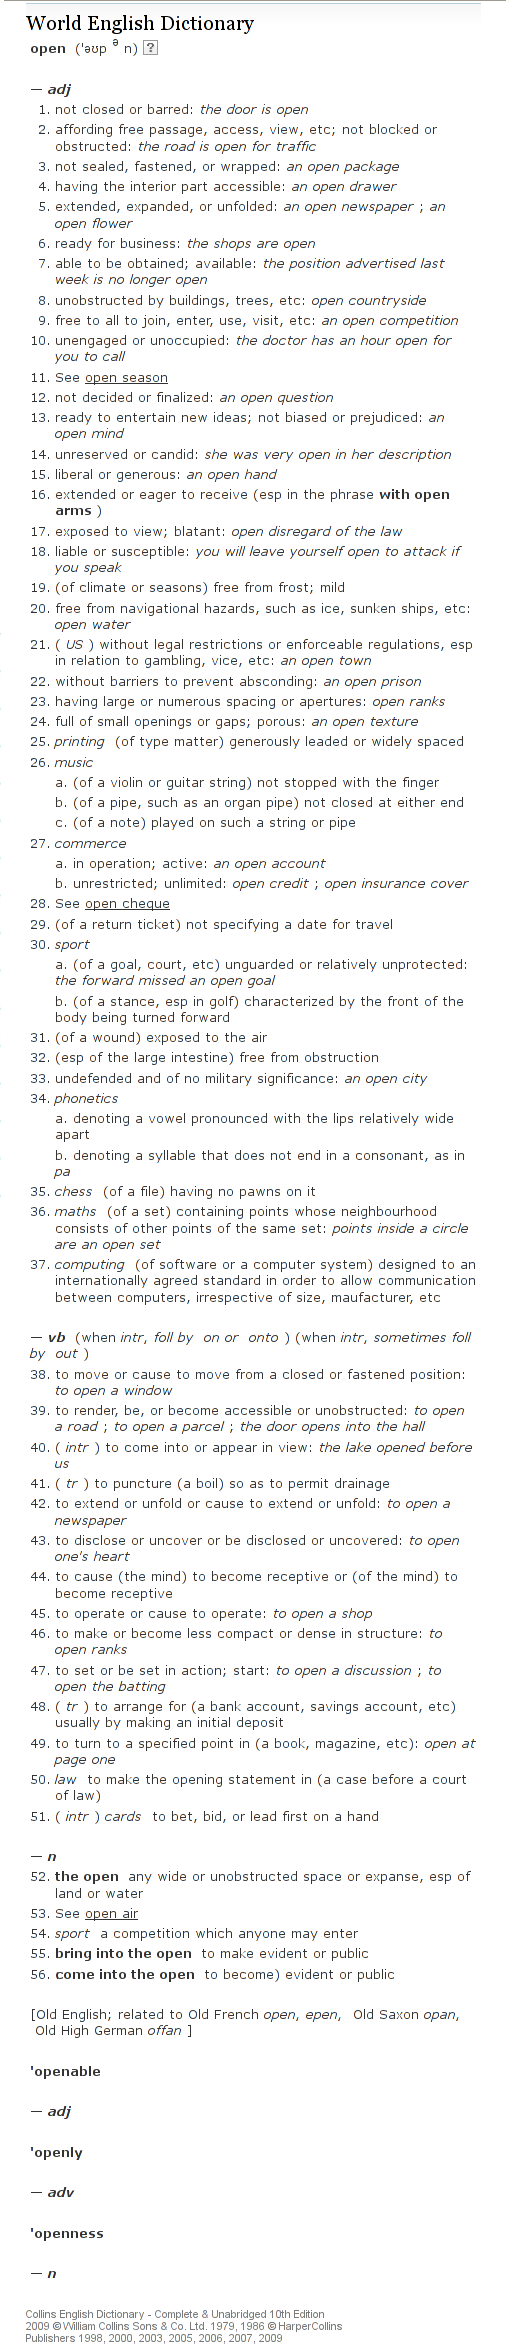
\includegraphics[height=0.8\textheight]{img/dictionary}\end{center}
\end{frame}

\begin{frame}
  \frametitle{What does the dictionary say?}
  \begin{center}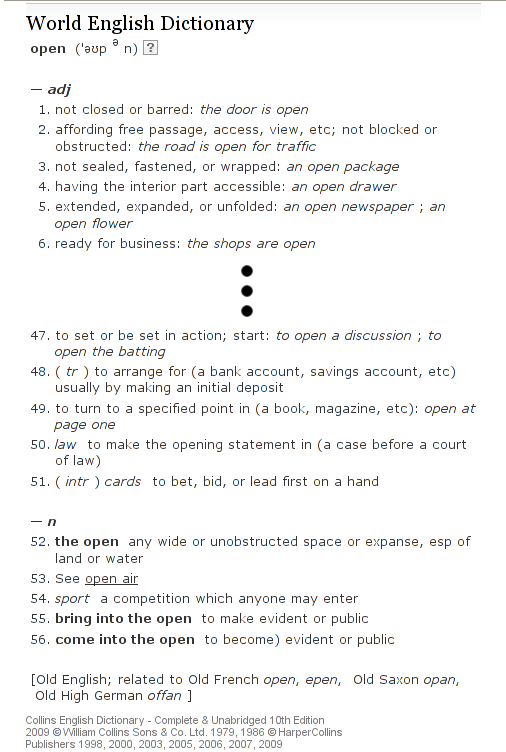
\includegraphics[height=0.8\textheight]{img/dictionary2}

    \href{http://dictionary.reference.com/browse/open}{http://dictionary.reference.com/browse/open}
  \end{center}
\end{frame}

\begin{frame}
  \frametitle{Our Definition}
  \begin{center}
    \begin{LARGE}
      The freedom to share, explore, reproduce, and contribute ideas and projects based on these ideas
    \end{LARGE}
\end{center}
\end{frame}

\begin{frame}
  \frametitle{Who, What, Where, When...}
  \begin{description}
  \item[Who uses and contributes to open projects?] Everyone, young and old!
  \item[What do they contribute?] Software, hardware, and content
  \item[Where do they do this from?] Anywhere in the world, thanks to the internet
  \item[When did this start?] 
  \end{description}
\end{frame}

\begin{frame}
  \frametitle{What can be open?}
  \begin{columns}
    \column{0.45\textwidth}
    \begin{center}
      \begin{LARGE}Software\end{LARGE}
      
      \vspace{5em}

      \begin{LARGE}Hardware\end{LARGE}

      \vspace{5em}

      \begin{LARGE}Content\end{LARGE}
    \end{center}
    \column{0.45\textwidth}
    \begin{center}
      
\includegraphics[width=0.4\textwidth]{img/opensource}

      \vspace{1em}

      
\includegraphics[width=0.4\textwidth]{img/opensourcehardware.png}

      \vspace{1em}

      
\includegraphics[width=0.8\textwidth]{img/cc.png}
    \end{center}
  \end{columns}

\end{frame}

\begin{frame}
  \frametitle{Formal Definition}
  \begin{center}
    \begin{block}{Software}
      Allows free distribution, modification the source code, allows
      derived works, does not discriminate or have limiting license
      restrictions\textemdash\textcolor{beamer@myblue}{\href{http://opensource.org/docs/osd}{opensource.org}}
    \end{block}

    \begin{block}{Hardware}
      hardware whose design is made publicly available so that anyone
      can study, modify, distribute, make, and sell the design or
      hardware based on that design\textemdash\textcolor{beamer@myblue}{\href{http://freedomdefined.org/OSHW}{OSHW}}
    \end{block}

    \begin{block}{Content}
      A piece of content or data is open if anyone is free to use,
      reuse, and redistribute it--subject only, at most, to the
      requirement to attribute and
      share-alike\textemdash\textcolor{beamer@myblue}{\href{http://www.opendefinition.org/}{opendefinition.org}}

      \vspace{1em}
      
      Open content encourages the 4Rs: Reuse, Revise, Remix,
      Redistribute\textemdash\textcolor{beamer@myblue}{\href{http://www.opencontent.org/definition/}{opencontent.org/definition}}
    \end{block}
  \end{center}
\end{frame}



\begin{frame}
  \frametitle{... and Why?}
\end{frame}

\begin{frame}
  \frametitle{Open vs. Proprietary}
  
  Proprietary
  \begin{itemize}
  \item May cost \textcolor{beamer@mygreen}{money} (not necessarily though!)
  \item \textcolor{beamer@mygreen}{Not} allowed to see how it works
  \item You're only \textcolor{beamer@mygreen}{licensed} to use it and don't own it
  \item Sometimes less \textcolor{beamer@mygreen}{secure}, as fewer experts get to look at how it was created
  \item May \textcolor{beamer@mygreen}{lock} users into a product that won't work with other systems once they've learned it
  \item Can add arbitrary \textcolor{beamer@mygreen}{restrictions} (like taking away features or keeping you from using it under arbitrary circumstances) to protect their product or get you to upgrade
  \end{itemize}

  \begin{block}{Remember}
    You can still sell open source software! Red Hat sells a distribution of Linux--but you can get the source code and get the exact same software for free.
  \end{block}

\end{frame}

\begin{frame}
  \frametitle{Open vs. Free vs. Free AND Open}

  Take software, for an example: 

  \begin{description}
  \item[Free Software] Freedom to do what you like with the software (e.g. give it away, create your own version, etc.)
  \item[Open Source] Ability to see how the software was created, and to share and improve it
  \item[Free Open Source Software / FOSS] A way to say both things at the same time!
  \item[Free Libre Open Source Software / FLOSS] Adds the ``libre'', which makes sure we know what kind of ``free'' we're talking about: free as in ``freedom'' not free as in no cost
  \end{description}

\end{frame}

\begin{frame}
  \frametitle{Software Examples}
  Examples of open projects:

  \begin{itemize}
  \item Software
    \begin{description}
    \item[Linux] Operating system that can be modified to work on just
      about any device
    \item[Firefox] Web browser that runs on any operating system (both
      open source operating systems and proprietary operating systems)
    \item[Open Office] Complete office suite that produces documents
      that can be opened by any system
    \item[Blender] 3D computer graphics software to model and render CGI images and video
    \end{description}
    \end{itemize}
\end{frame}

\begin{frame}
  \frametitle{Linux}
  \begin{columns}
    \column{0.45\textwidth}
    \begin{LARGE}
      Linux
    \end{LARGE}
    \begin{itemize}
    \item Released in 1991 by Linux Torvalds
    \item Created as a free alternative to Unix
    \item Now runs on
      \begin{itemize}
      \item MACs \& PCs
      \item Video game consoles
      \item PDAs and Phones (Android)
      \item GPSs and Cars
      \item Servers / Supercomputers
      \end{itemize}
    \end{itemize}
    \column{0.45\textwidth}
      \begin{center}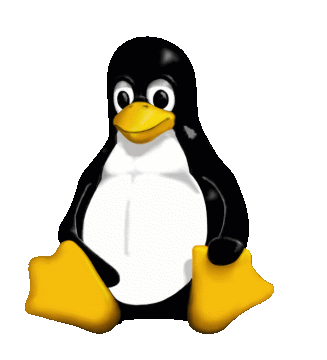
\includegraphics[width=0.5\textwidth]{img/tux}\end{center}
      
      \begin{center}
\includegraphics[width=0.5\textwidth]{img/ubuntu}\end{center}
  \end{columns}
\end{frame}

\begin{frame}
  \frametitle{Who Contributes to Linux?}
  All of these companies actively work to make Linux better (and since Linux is Open Source, we all get to benefit from their work):
  \begin{columns}
    \column{0.45\textwidth}
    
    \begin{Large}
      \begin{itemize}
      \item Red Hat
      \item Novell
      \item IBM
      \item Intel
      \item Oracle
      \item Google
      \item $\ldots$
        even 
\includegraphics[width=0.3\textwidth]{img/microsoft}!
      \end{itemize}
    \end{Large}

    \column{0.45\textwidth}
    \begin{center}
      
\includegraphics[width=0.3\textwidth]{img/redhat}

      
\includegraphics[width=0.4\textwidth]{img/novell}

      
\includegraphics[width=0.3\textwidth]{img/ibm}

      
\includegraphics[width=0.3\textwidth]{img/intel}

      
\includegraphics[width=0.4\textwidth]{img/oracle}

      
\includegraphics[width=0.4\textwidth]{img/google}
    \end{center}
  \end{columns}
  \begin{center}
    You've used Linux if you've ever Googled anything!
  \end{center}

\end{frame}

\begin{frame}
  \frametitle{Blender}
  \begin{center}
    
\includegraphics[width=0.8\textwidth]{img/blenderex}
  \end{center}
  \begin{itemize}
  \item Fully featured 3D modeler, renderer, and compositer
  \item Works on all major operating systems, and even on old hardware
    \\ (I was using blender back in 2001!)
  \item Is free, compared to commercial software that cost 1000s of
    dollars, so anyone can start learning how to use it right away
  \item Has state-of-the-art features comparable to similar
    proprietary tools--you can do studio-quality work in Blender!
  \end{itemize}
\end{frame}

\begin{frame}
  \frametitle{Blender Example}
    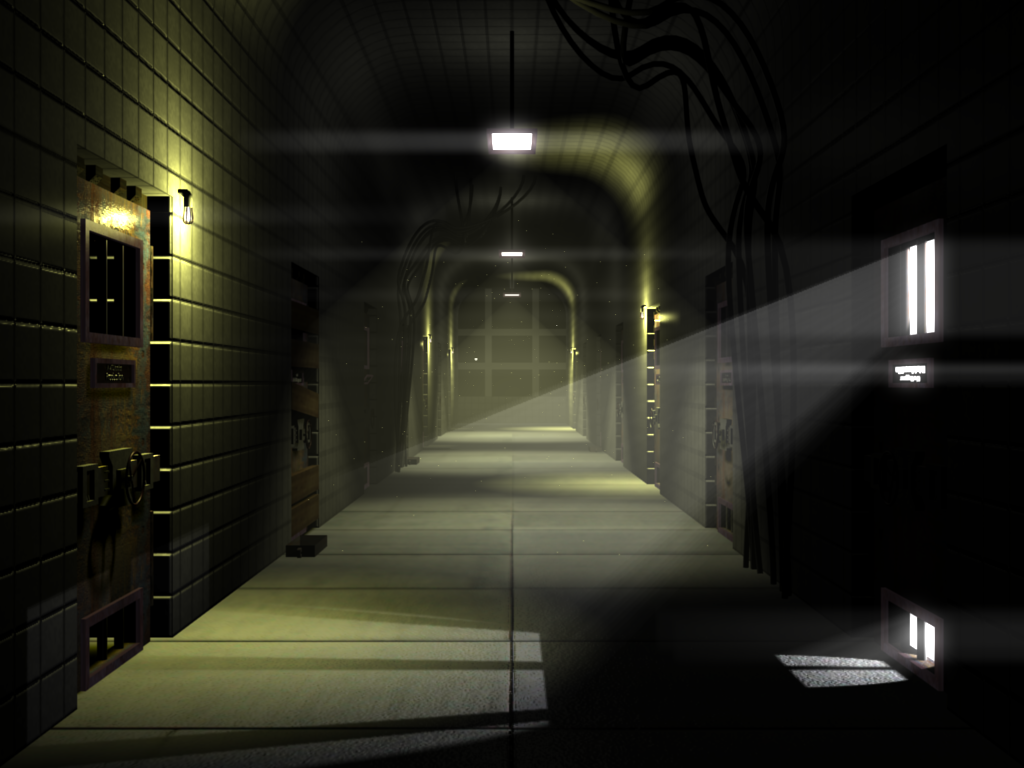
\includegraphics[width=\textwidth]{img/blendermine}
\end{frame}

\begin{frame}
  \frametitle{Hardware Examples}
  Examples of open projects:

  \begin{itemize}
  \item Hardware
    \begin{description}
    \item[OpenCola] A softdrink that can be made by anyone (the recipe
      is available) so there are no hidden ingredients that might be
      unhealthy or dangerous
    \item[Makerbot Thing-O-Matic] A \textcolor{beamer@myblue}{3D}
      Printer that can produce 3D objects out of a special
      plastic--can not only be built by anyone if they have the parts,
      but can \textcolor{beamer@myblue}{reproduce} itself by printing
      the necessary components to build a new device.
    \end{description}
  \end{itemize}
\end{frame}

\begin{frame}
  \frametitle{Content Examples}
  Examples of open projects:
  \begin{itemize}
  \item Content
    \begin{description}
    \item[Wikipedia] An online encyclopedia that can be freely accessed (and modified!) by anyone
    \item[Project Gutenberg] An archive of public domain content that is made available in long-lasting open formats that 
    \end{description}
  \end{itemize}
\end{frame}

\end{document}
